\chapter{Result}\label{cha:result}

This Chapter first describes the experiment to evaluate the algorithm and then presents the results.

\section{Experiment}
%{and FRGC database CITE}
To evaluate the algorithm, a set of 106 images of faces en face were acquired from SCface database \cite{SCface}. Facial marks of interest were marked and labeled as a permanent or a non-permanent by the supervisors at NFC. This resulted in 506 marks where 353 were permanent and 153 were non-permanent.

The experiment was set such that the image set was processed by the algorithm with 11 different thresholds values, $h_{FRS}$, for the FRS-image. The $h_{FRS}$ ranged from $0.05$ to $0.15$. The output was compared to the ground truth. A correct detection was defined as all detections which had a union with an annotated mark. This definition has been chosen since some of the detections can be very small. Also, since candidates larger than 1000 pixels has been eliminated, no over large candidates can give correct detections.   

The evaluation measurement for the detector is the precision \eqref{eq:precision} and recall \eqref{eq:recall} value. Precision tells how well the detector is to avoid false detections while recall tells how well it finds the annotated marks. The result from the different $h_{FRS}$-values can be seen in \cref{fig:results_bar_frs}.

\begin{equation} \label{eq:precision}
Precision = \frac{\text{Number of correct detections}}{\text{Number of detections}}
\end{equation}
\begin{equation} \label{eq:recall}
Recall = \frac{\text{Number of correct detections}}{\text{Number of annotated marks}}
\end{equation}

The $h_{FRS}$-value which gives the best recall value was used to evaluate the elimination process of the candidates. This was done by calculating the precision and recall values before the different elimination steps. The results is displayed in \cref{fig:results_bar_frs}.

To evaluate the facial mark classifier, a cross validation of the 506 annotated mark were performed. 25 marks was chosen at random to be used as test marks while the remaining marks was used for training the SVM. This was repeated until all the marks had been used as test marks.

In order to find the best $C$-value and $\gamma$-value for the mark classifier, the parameters are varied over a rough interval to narrow down the search. Afterwards, a more fine interval is used to find the best parameters. This has been shown by Chih-Wei et. al. \cite{svm_guide}  to be an effective method compared to a more random selection of parameters which is often used by people unfamiliar to SVM. 

\section{Results from experiment}

In the \cref{fig:results_bar_frs}, the precision and recall for different $h_{FRS}$-value can be examined. The precision corresponds to the white bar and the recall corresponds to the black bar. Note that this is only the detections of facial mark and no classification between permanent and non-permanent marks. 

\begin{figure}[h!]
	\centering
	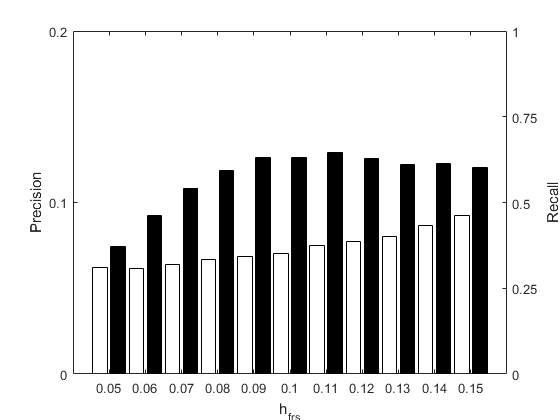
\includegraphics[width=\textwidth*3/4,height=\textheight*3/4,keepaspectratio]{results_bar_frs}
	\caption{Detection results from the algorithm with different $h_{frs}$-values. The white bars represent the precision value and the black bars represent recall value.  \label{fig:results_bar_frs}}
\end{figure}

As one can see, the precision increases with higher $h_{FRS}$-value without affecting the recall substantially. This is means that the number of candidates decreases with a growing $h_{FRS}$-value. Thus, a small $h_{FRS}$-value results in a large amount of candidates while a larger value gives fewer candidates.

In \cref{fig:results_bar_elimniation}, it is possible to see the effects of the different elimination steps. As before, the white bar represent the precision and the black bar represent the recall. The first pair is the result just after the candidate detection and the second pair is the result after the blob detector. Furthermore, the third pair is after the hair eliminator and the last pair is after the size eliminator. 

\begin{figure}[h!]
	\centering
	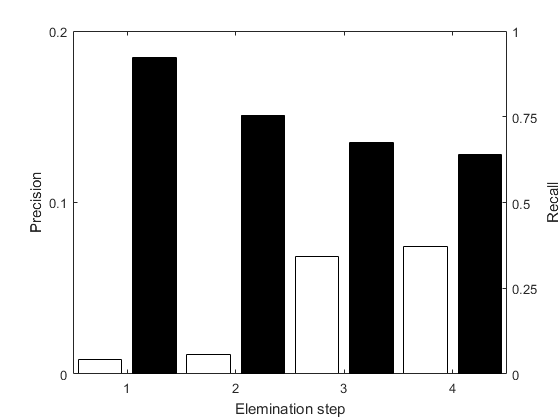
\includegraphics[width=\textwidth*3/4,height=\textheight*3/4,keepaspectratio]{results_bar_elimniation}
	\caption{Detection results from the algorithm  after different candidate elimination steps. 1 = before elimination, 2 = after blob-elimination, 3 = after hair-elimination, 4 = after size-elimination. The white bars represent the precision value and the black bars represent recall value.  \label{fig:results_bar_elimniation}}
\end{figure}

It is obvious that the different eliminators are essential for the algorithm. The hair eliminator improves the precision the most while the blob detector worsen the recall the most.     




%The result from the classifier can be presented as a confusion matrix, see \cref{table:confusion_mat}. A positive result is a permanent mark and a negative result is a non-permanent mark. The accuracy of the classifier is $83\%$ 

%\begin{table}[h!]
%\begin{center}
%	\caption{Confusion matrix from RPPVS classifier}
%	\begin{tabular}{|c|c|c|}
%		\hline
%		                 & Predicted positive & Predicted negative \\ \hline
%		Labeled positive &        321         &        32         \\ \hline
%		Labeled negative &         54         &        99         \\ \hline
%
%	\end{tabular}
%
%\label{table:confusion_mat}
%\end{center}
%\end{table}
\newpage
The result from the mark classifier is presented as accuracy matrix with varying $C$-value and $\gamma$-value. The accuracy is calculated as in \eqref{eq:accuracy}. In \cref{fig:crude_acc}, the $C$-value ranges from $1$ to $100$ while the $\gamma$-value ranges from $10^{-2}$ to $1$.

\begin{equation} \label{eq:accuracy}
Accuracy [\%] = \frac{\text{True positive} + \text{True negative}}{\text{Number of annotated marks}}
\end{equation}

\begin{figure}[h!]
	\centering
	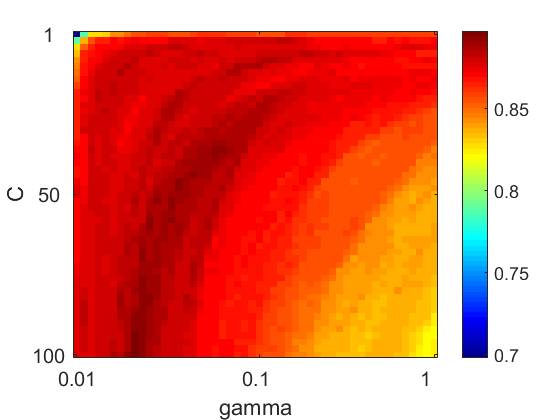
\includegraphics[width=\textwidth*3/4,height=\textheight*3/4,keepaspectratio]{crude_acc_2}
	\caption{Crude accuracy matrix where $1 \leq \gamma \leq 100$ and $10^{-2} \leq \gamma \leq 1$.
		 \label{fig:crude_acc}}
\end{figure}

 As show, the best accuracy is when $C \approx 95$ and $\gamma \approx 5*10^{-2}$. Therefore, with a finer interval for the two parameters, \cref{fig:fine_acc} was generated. Here, the $C$-value ranges from $90$ to $115$ while the $\gamma$-value ranges from $5*10^{-2}$ to $2*10^{-1}$. 

\begin{figure}[h!]
	\centering
	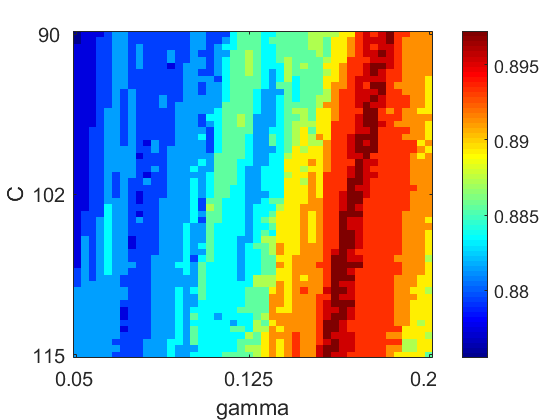
\includegraphics[width=\textwidth*3/4,height=\textheight*3/4,keepaspectratio]{fine_acc_2}
	\caption{Fine accuracy matrix where $90 \leq \gamma \leq 115$ and $5*10^{-2} \leq \gamma \leq 2*10^{-1}$.
		 \label{fig:fine_acc}}
\end{figure}

Form \cref{fig:fine_acc} it is possible to conclude that the best accuracy is acquired with several pair of parameters and results in the accuracy 90\%. $C = 100$ and $\gamma = 0,14$ is one of those pairs. Therefore, the mark classifier is given these values as parameters for the SVM. 


